%!TEX root = Thesis_main.tex
\chapter{Introduction}
\label{chapter1}

\section{Overview}
In the last decades industry is being moving from the use of traditional robotic arms (manipulators), which executes highly specific simple tasks in controlled and secure environments, like spot welding, towards more complex and flexible robotic systems, which should be able to cope with dynamic and uncertain environments. \\ 
Even before industrial robot manipulators, in the '50s, the idea of building mobile systems that can move autonomously in unstructured environments was raising. The first was William Grey Walter who built a couple of mobile vehicles with already embedded sensors to avoid obstacles, then in 1969 the mobile robot SHAKEY has been developed in Stanford University, named after its shaking behaviour to move towards an object which it could recognise, then the JPL Rover for space exploration has been developed in the '70s, and so on until nowadays where different types of robots can be found in a great variety of environments, ranging from the cleaning robots in people houses, to legged mobile robots inspired to animal behaviour.
\begin{figure}[h!]
	\centering
	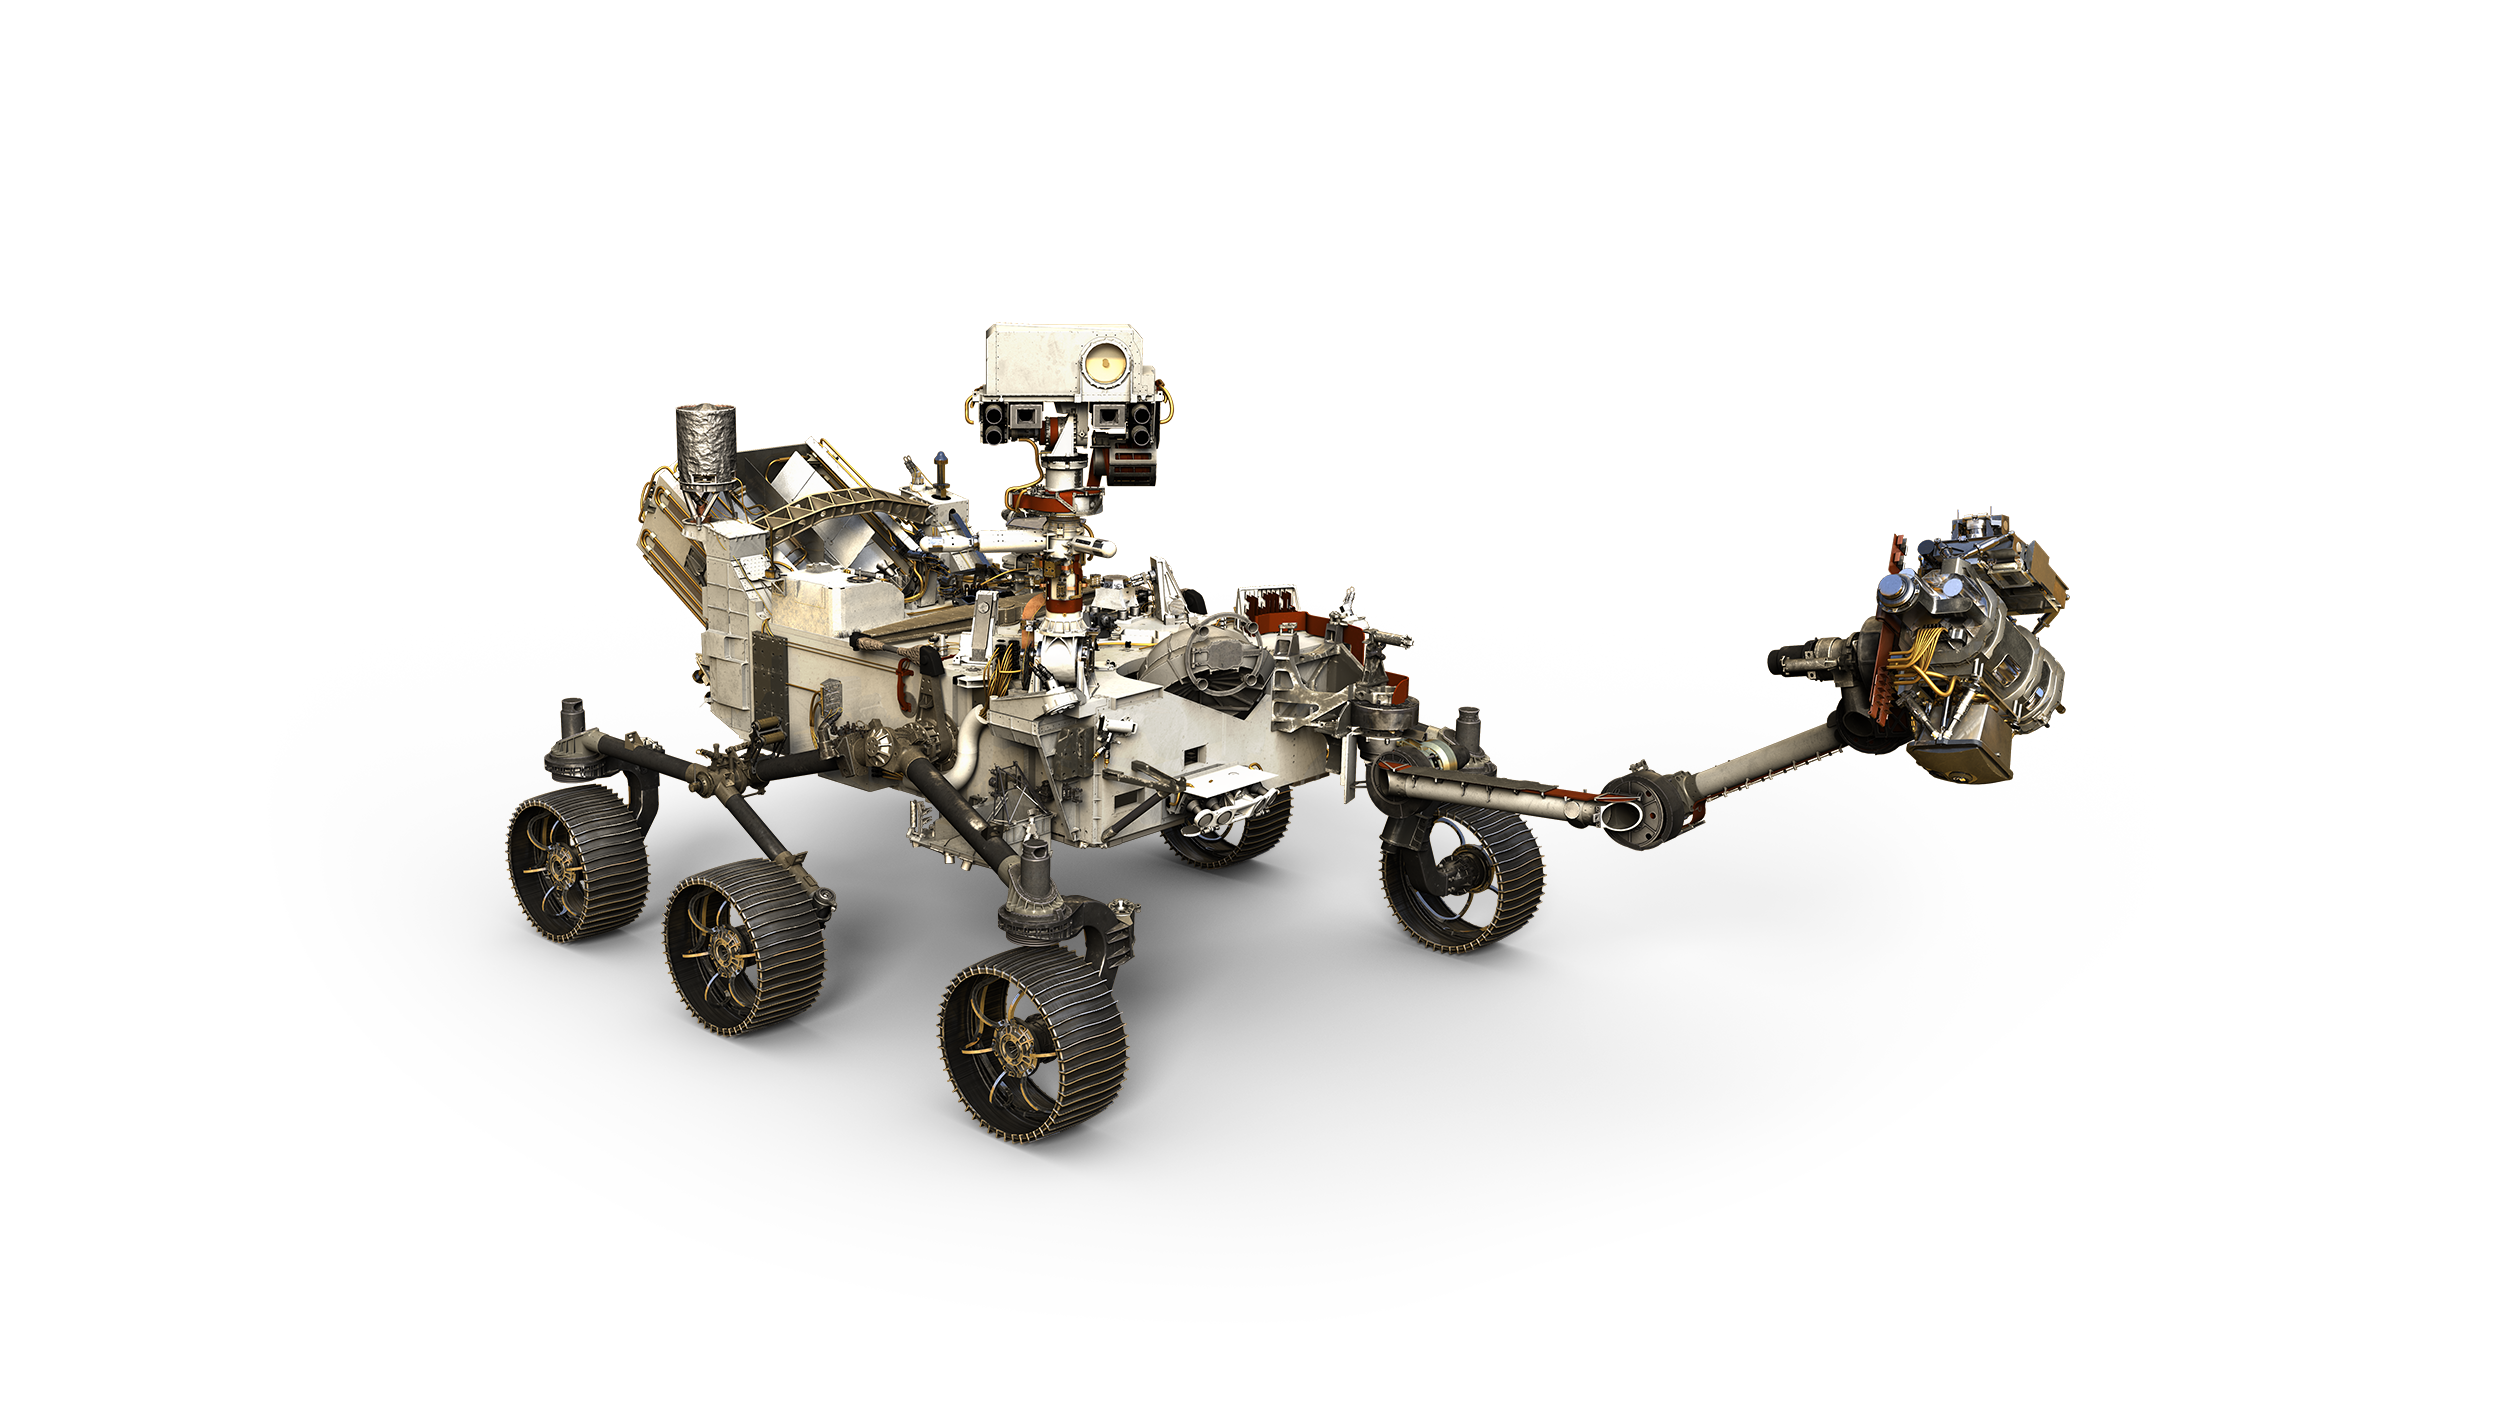
\includegraphics[scale=0.15]{JPL_rover}
	\caption{JPL Rover designed for Mars2020 mission}
\end{figure}
In industry too automated robotic systems are used in order to achieve:
\begin{itemize}
	\item A better production quality, having the possibility to more easily measure and control the performances;
	\item Improved productivity, reducing downtimes and the consumption of resources;
	\item Robots can have access to environments which are too risky or not accessible for humans;
	\item Robots maintenance can be much cheaper than other man-driven alternatives. 
\end{itemize}
In this sense mobile robotics is a very practical example of how the efficiency of a plant can be improved, reducing the effort for the trasportation tasks, or collecting datas from a warehouse automatically, or in many other ways.\\
However, when in the early '90s people has started mounting manipulator arms on mobile platforms, the resulting system opened the research to endless possibilities. These systems are now called Mobile Manipulators.
The mobility of robots substantially increased what they can cope. Robots are now expected to explore unknown dynamic environments, interact with human beings or manipulate hazardous products. Mobile manipulators are systems that combine locomotion and manipulation capabilities in order to fulfil such missions. \\
Except for some special types of Mobile Manipulators like:
\begin{itemize}
	\item Submarine Mobile Manipulators for underwater applications;\begin{figure}[h!]
		\centering
		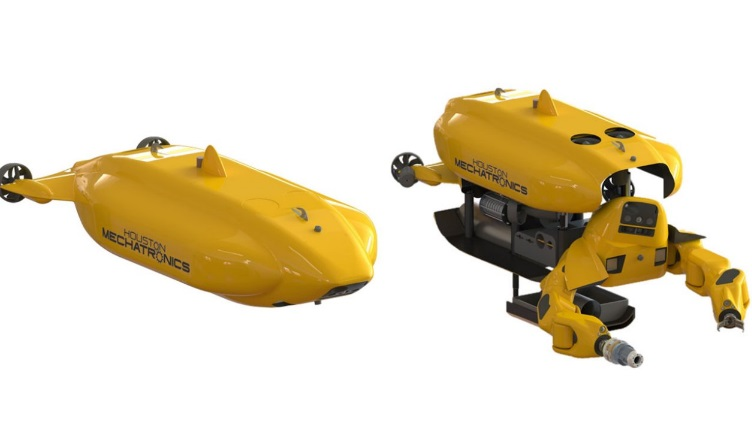
\includegraphics[scale=0.3]{submarine_robot}
		\caption{Houston Mechatronics's Aquanaut}
		\label{fig:aquanaut} 
	\end{figure}
	\item Legged humanoid or animal-like robots for service missions;\begin{figure}[h!]
		\centering 
		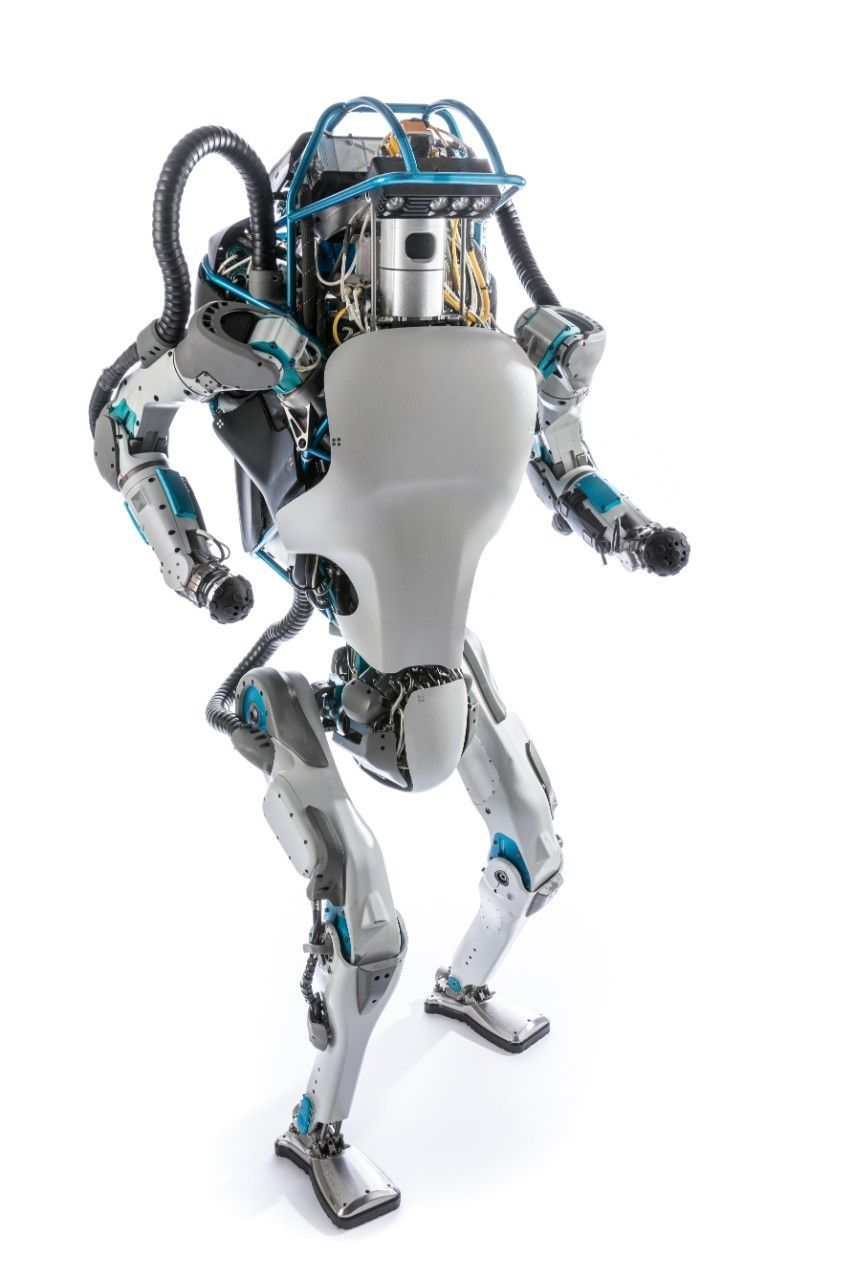
\includegraphics[scale=0.095]{atlas}
		\label{fig:atlas} 
		\quad
		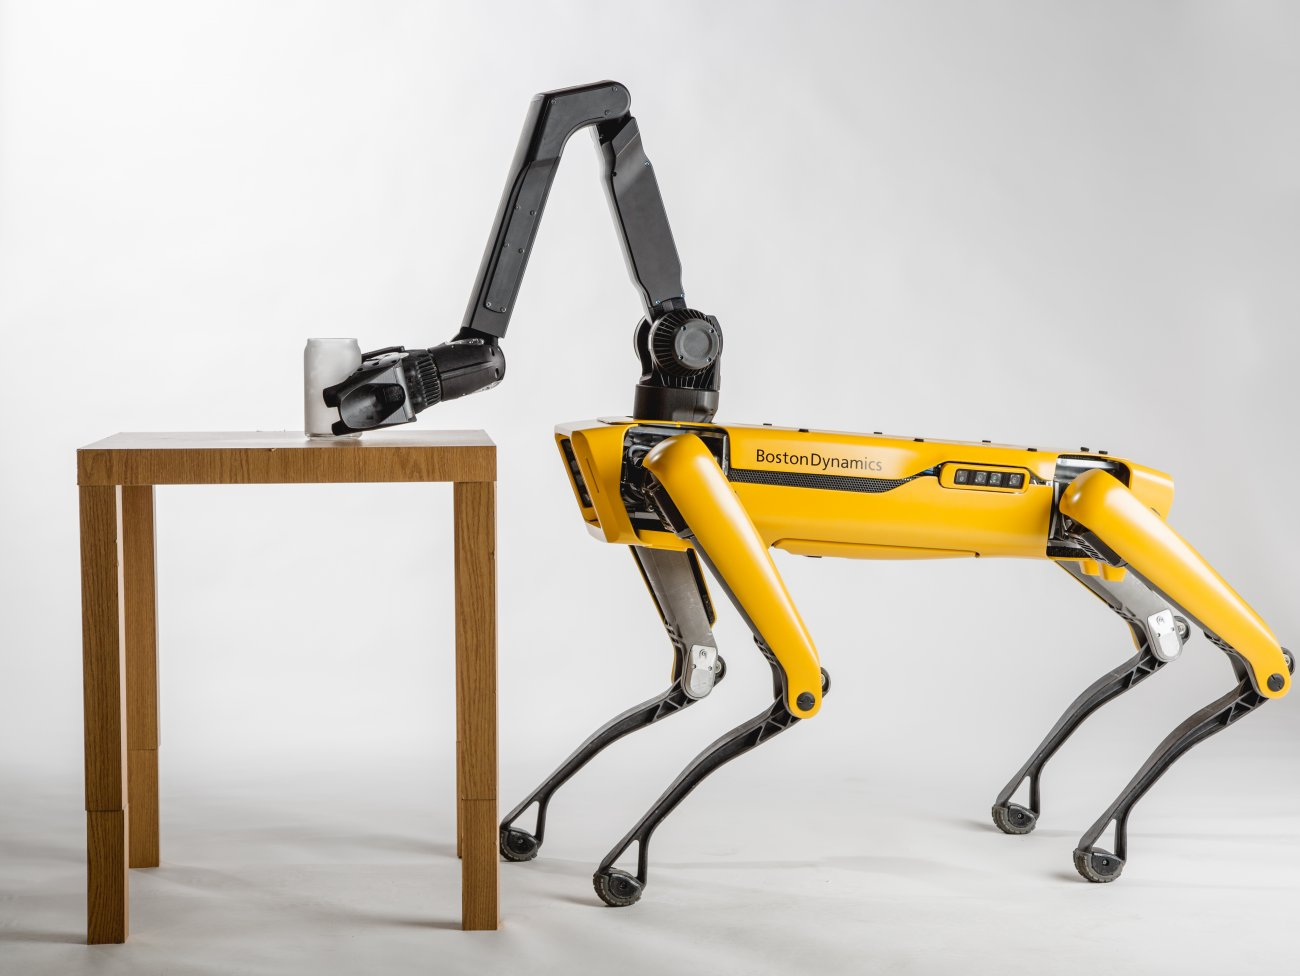
\includegraphics[scale=0.10]{spot_mini}
		\label{fig:spotmini} 
		\caption{Boston Dynamics's Atlas and Spot Mini}
	\end{figure}
	\item Omnidirectional vehicles \begin{figure}[h!]
		\centering
		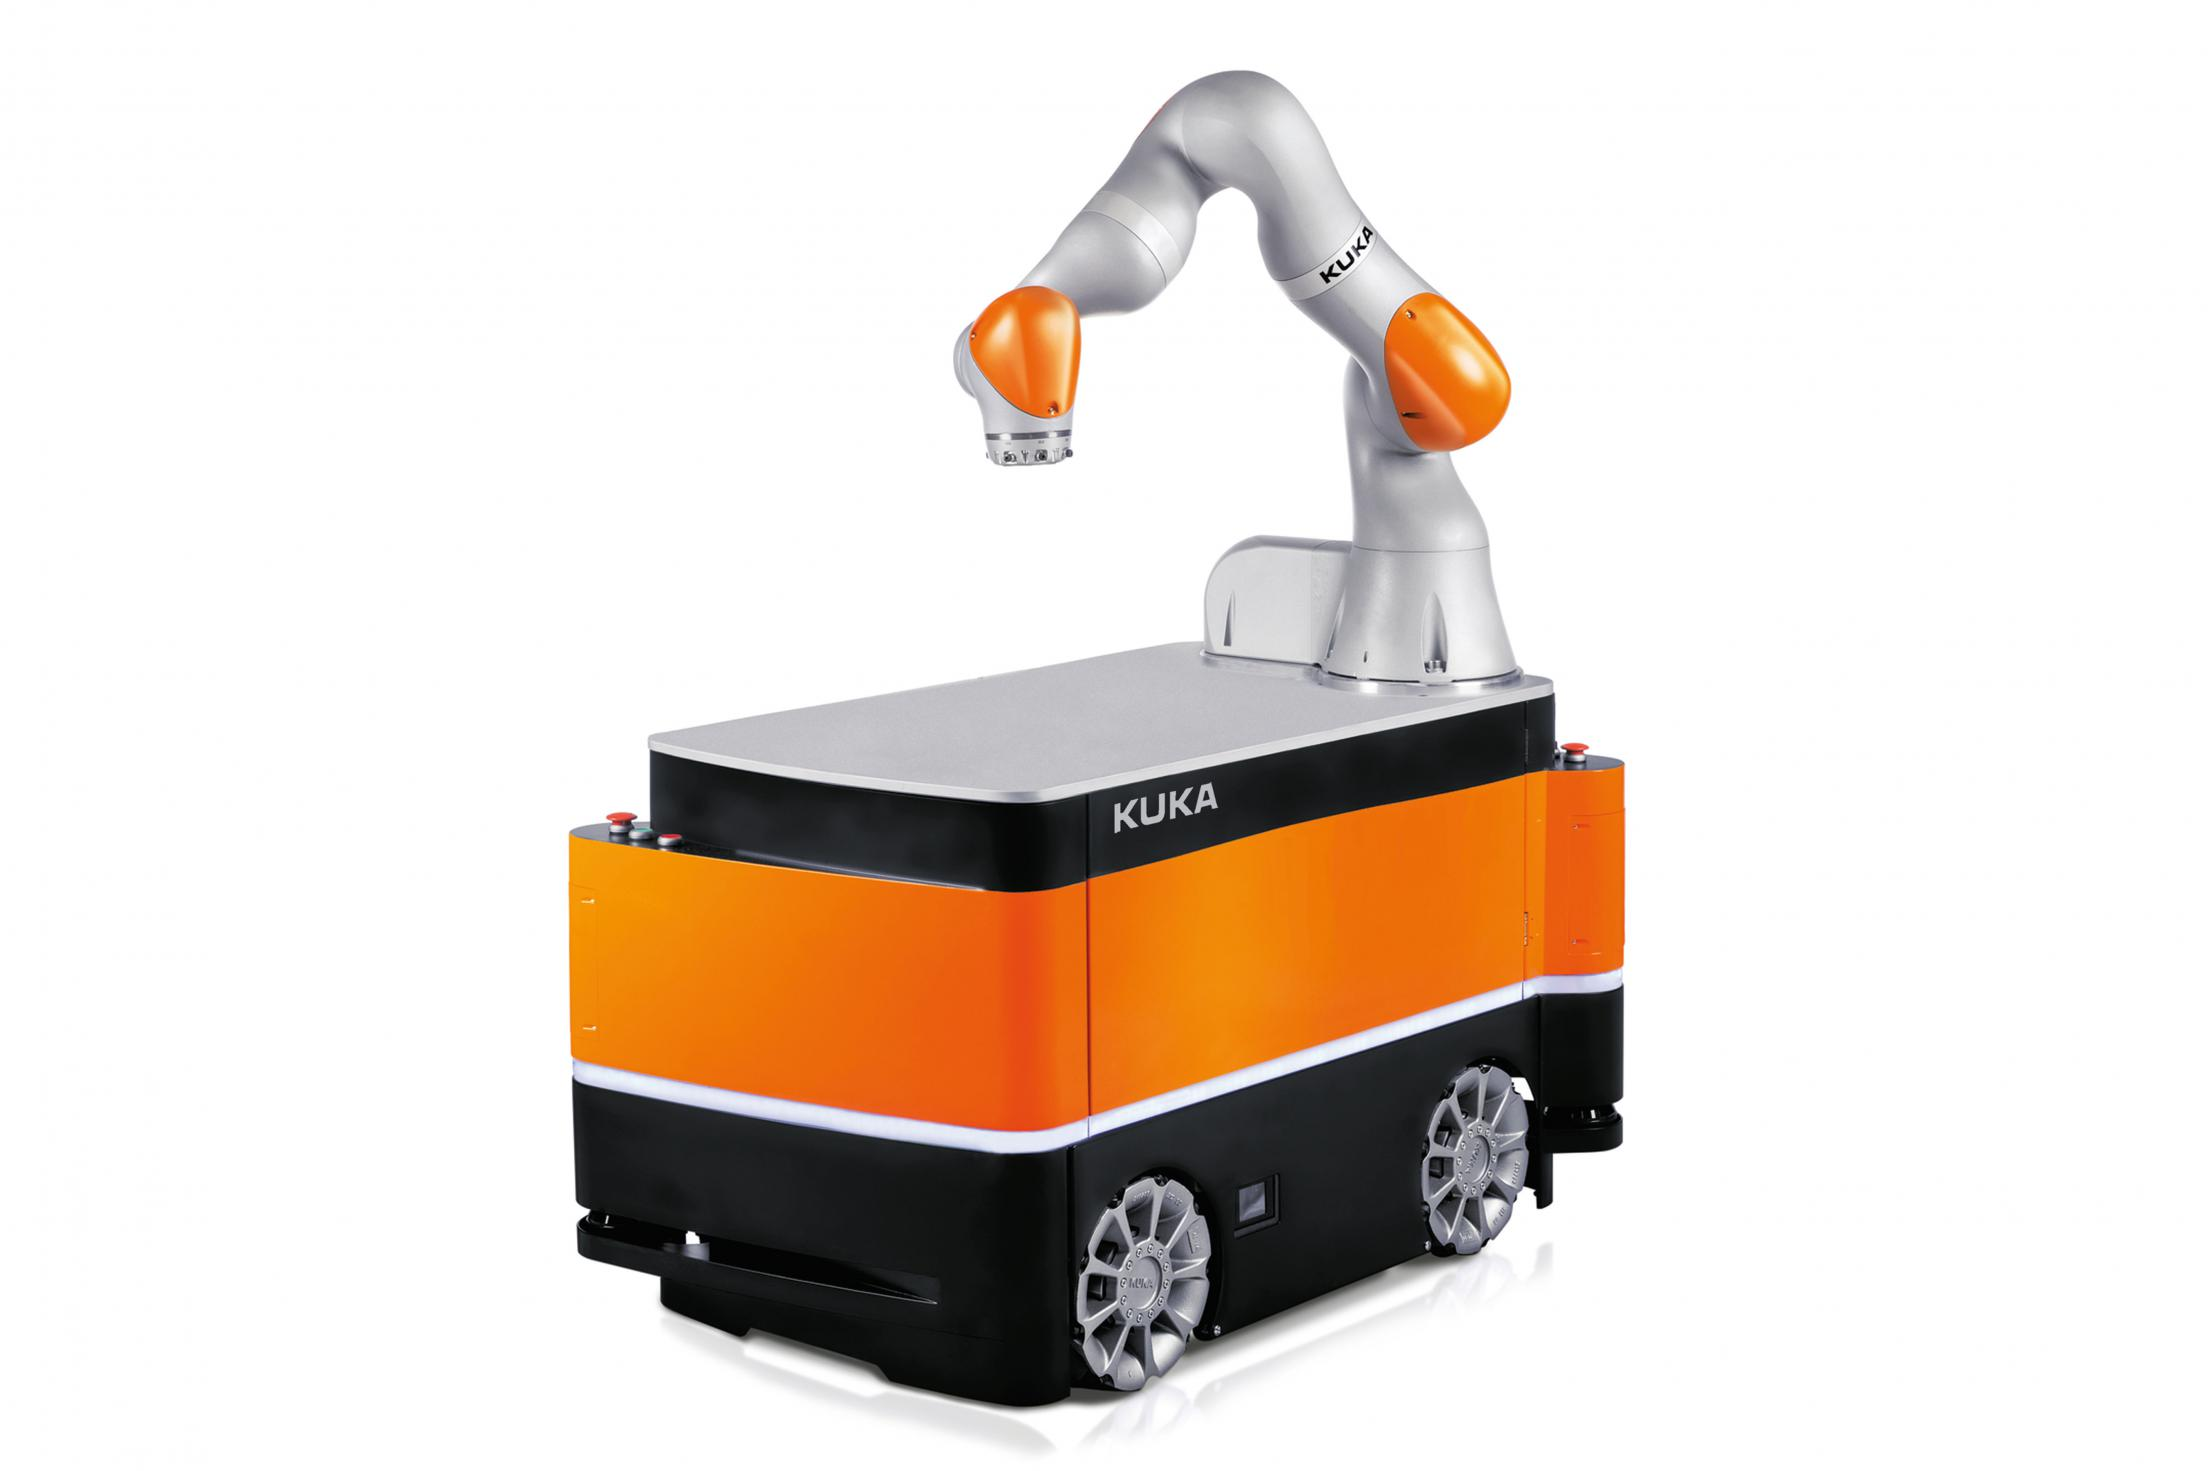
\includegraphics[scale=0.095]{kuka_iiwa}
		\caption{Kuka KMR iiwa: a Mobile Manipulator with omnidirectional wheels}
		\label{fig:iiwa} 
	\end{figure}
\end{itemize}
Mobile Manipulators combine a nonholonomic wheeled mobile base and one or more robotic arms. From a physical point of view the presence of the base makes the entire Mobile Manipulator a nonholonomic system, meaning a system described by a set of variables subjected to differential constraints. Nonholonomic constraints will be better explained in Chapter \ref{chapter2}. The same chapter is also devoted to the kinematic and dynamic description of wheeled Mobile Manipulators, mainly pointing to two important aspects:
\begin{enumerate}
	\item The entire system is often kinematically redundant with respect to the task to be achieved;
	\item The dynamic properties of the base are very different from the manipultor ones.
\end{enumerate}
After a brief introduction about the theory of control strategies in Chapter \ref{chapter3}, Chapter \ref{chapter4} can be referred for a fairly thorough summary of Mobile Manipulator control; even if Mobile Manipulators are a technology known from the early 90s, just a little can be found in literature on this topic. In particular, except for very few cases, MPC control has been applied only with holonomic Mobile Manipulators. This is due to the fact that this kind of control requires high computational effort, especially with highly nonlinear systems like Mobile Manipulators. MPC is a powerful tool to face all the constraints on Mobile Manipulators motion that have to be taken into account: obstacle avoidance, self collision avoidance, joint limits, joint speed limits, singular configurations avoidance, etc. exploiting also the kinematic redundancy of the system.\\
In Chapter \ref{chapter5} we present the architecture of an online MPC control for a nonholonomic Mobile Manipulator in order to achieve a trajectory following task for the manipulator's end effector while coping with the constraints previously mentioned. In Chapter \ref{chapter6} experimental results are presented and eventually in Chapter \ref{chapter7} conclusions are drawn highlighting our main contributions and future work.	

\section{Objective of the thesis}
The main objective of this thesis is to design a controller for a Nonholomic Mobile Manipulator able to perform trajectory tracking for motion and grasping operations in unstructured enviroments. The trajectories are given as end effector position and orientation in time in order to perform grasping of objects in a time-optimal manner. The planning algorithm presented in \cite{shantanuthakar} precomputes the optimal trajectories to perform a specific task, although the algoritm is not suitable for online implementation because of the high execution time. The design of an online controller is then required, also to take into account unexpeted events and positioning errors of the end effector. The main issue related to the developement of such a controller lies in the non linearity of the model and the high redundancy of the system itself. For those reasons a control technique that allows to take into account unforseen events, manipulability and constraints on the system has to be identified. The complexity of the problem and the variety of tasks requires to use a hierarchical approach and, given that low level loops are provided by manufacurers, to find a suitable high level control logic. The field of control for mobile manipulator is nowdays of great interest because of the increased possibilities and requirements in industrial applications.  



